\documentclass[11pt,a4paper]{article}
\usepackage[margin=0.75in]{geometry}
\usepackage{graphicx}
\usepackage{authblk}
\usepackage{subcaption}
\author[1]{Santiago Acosta\thanks{santiago\_acosta@ucsb.edu}}
\author[1]{Jonathan Skaza\thanks{skaza@ucsb.edu}}
\affil[1]{Dynamical Neuroscience Graduate Program, University of California, Santa Barbara}
\title {Neural Population Geometry \\[1ex] \large ME 225NN, Winter 2025}
\date{}

\begin{document}
\maketitle
\section{Introduction}

\subsection{Problem Description \& Motivation}
Experimental neuroscience has seen rapid advances in recording techniques, with the ability to record from thousands of (and possibly a million~\cite{demas2021high}) neurons simultaneously. In the realm of theoretical neuroscience, these advancements have sparked a concerted effort toward the development of methodologies for the analysis of neural systems or populations of neurons. Studying large neural populations presents a unique set of challenges, as neurons often respond to multiple variables at once, making their roles more difficult to interpret. Additionally, real-world tasks require robustness to complex variability, which may limit the usefulness of traditional tuning-based analyses.

In consideration of these factors, the focus of neural population analysis has transitioned from single-neuron tuning to geometric approaches that consider population-level representations~\cite{yuste2015neuron, saxena2019towards}. The rationale behind this shift is that neural computations arise from structured, high-dimensional activity patterns rather than isolated responses of individual neurons. These patterns have been cleverly conceptualized as \textit{neural manifolds}---low-dimensional geometric structures embedded in high-dimensional neural state space. The properties of these manifolds, including their dimensionality, curvature, and separability, as well as the manifold capacity---the number of manifolds a neural system can support, provide insights into the computational principles governing networks of neurons~\cite{chung2021neural}.

This report centers around the application of geometric techniques in the analysis of large populations of neurons, a field referred to as \textit{neural population geometry}. Importantly, this framework provides a unified approach for understanding both biological neural circuits and artificial neural networks (ANNs). By framing neural computation in terms of geometric transformations, we can analyze how population-level representations contribute to robust, efficient, and scalable information processing across both biological and artificial systems. This parallel analysis may help reveal similarities in how these different types of neural networks organize and process information.

\subsection{Literature Review}
\subsection{Summary}
Neural population geometry provides a powerful framework for analyzing large-scale neural activity by leveraging geometric principles to describe population-level representations. This approach has yielded mechanistic insights into various domains, including perception, decision-making, motor control, and cognition. By examining the structure and transformations of neural manifolds, researchers have uncovered fundamental constraints and computational strategies underlying neural function.

Moreover, the study of neural population geometry bridges biological and artificial neural networks (ANNs), revealing shared representational structures that support efficient and generalizable computation. In both domains, geometric properties such as dimensionality, curvature, and separability shape the ability of neural systems to encode and process information. By adopting a geometric perspective, we gain a deeper understanding of how neural populations achieve robustness, efficiency, and scalability in complex tasks.

\section{Preliminaries}
\subsection{Neural State Space \& Population Activity}
\begin{figure}
    \centering
    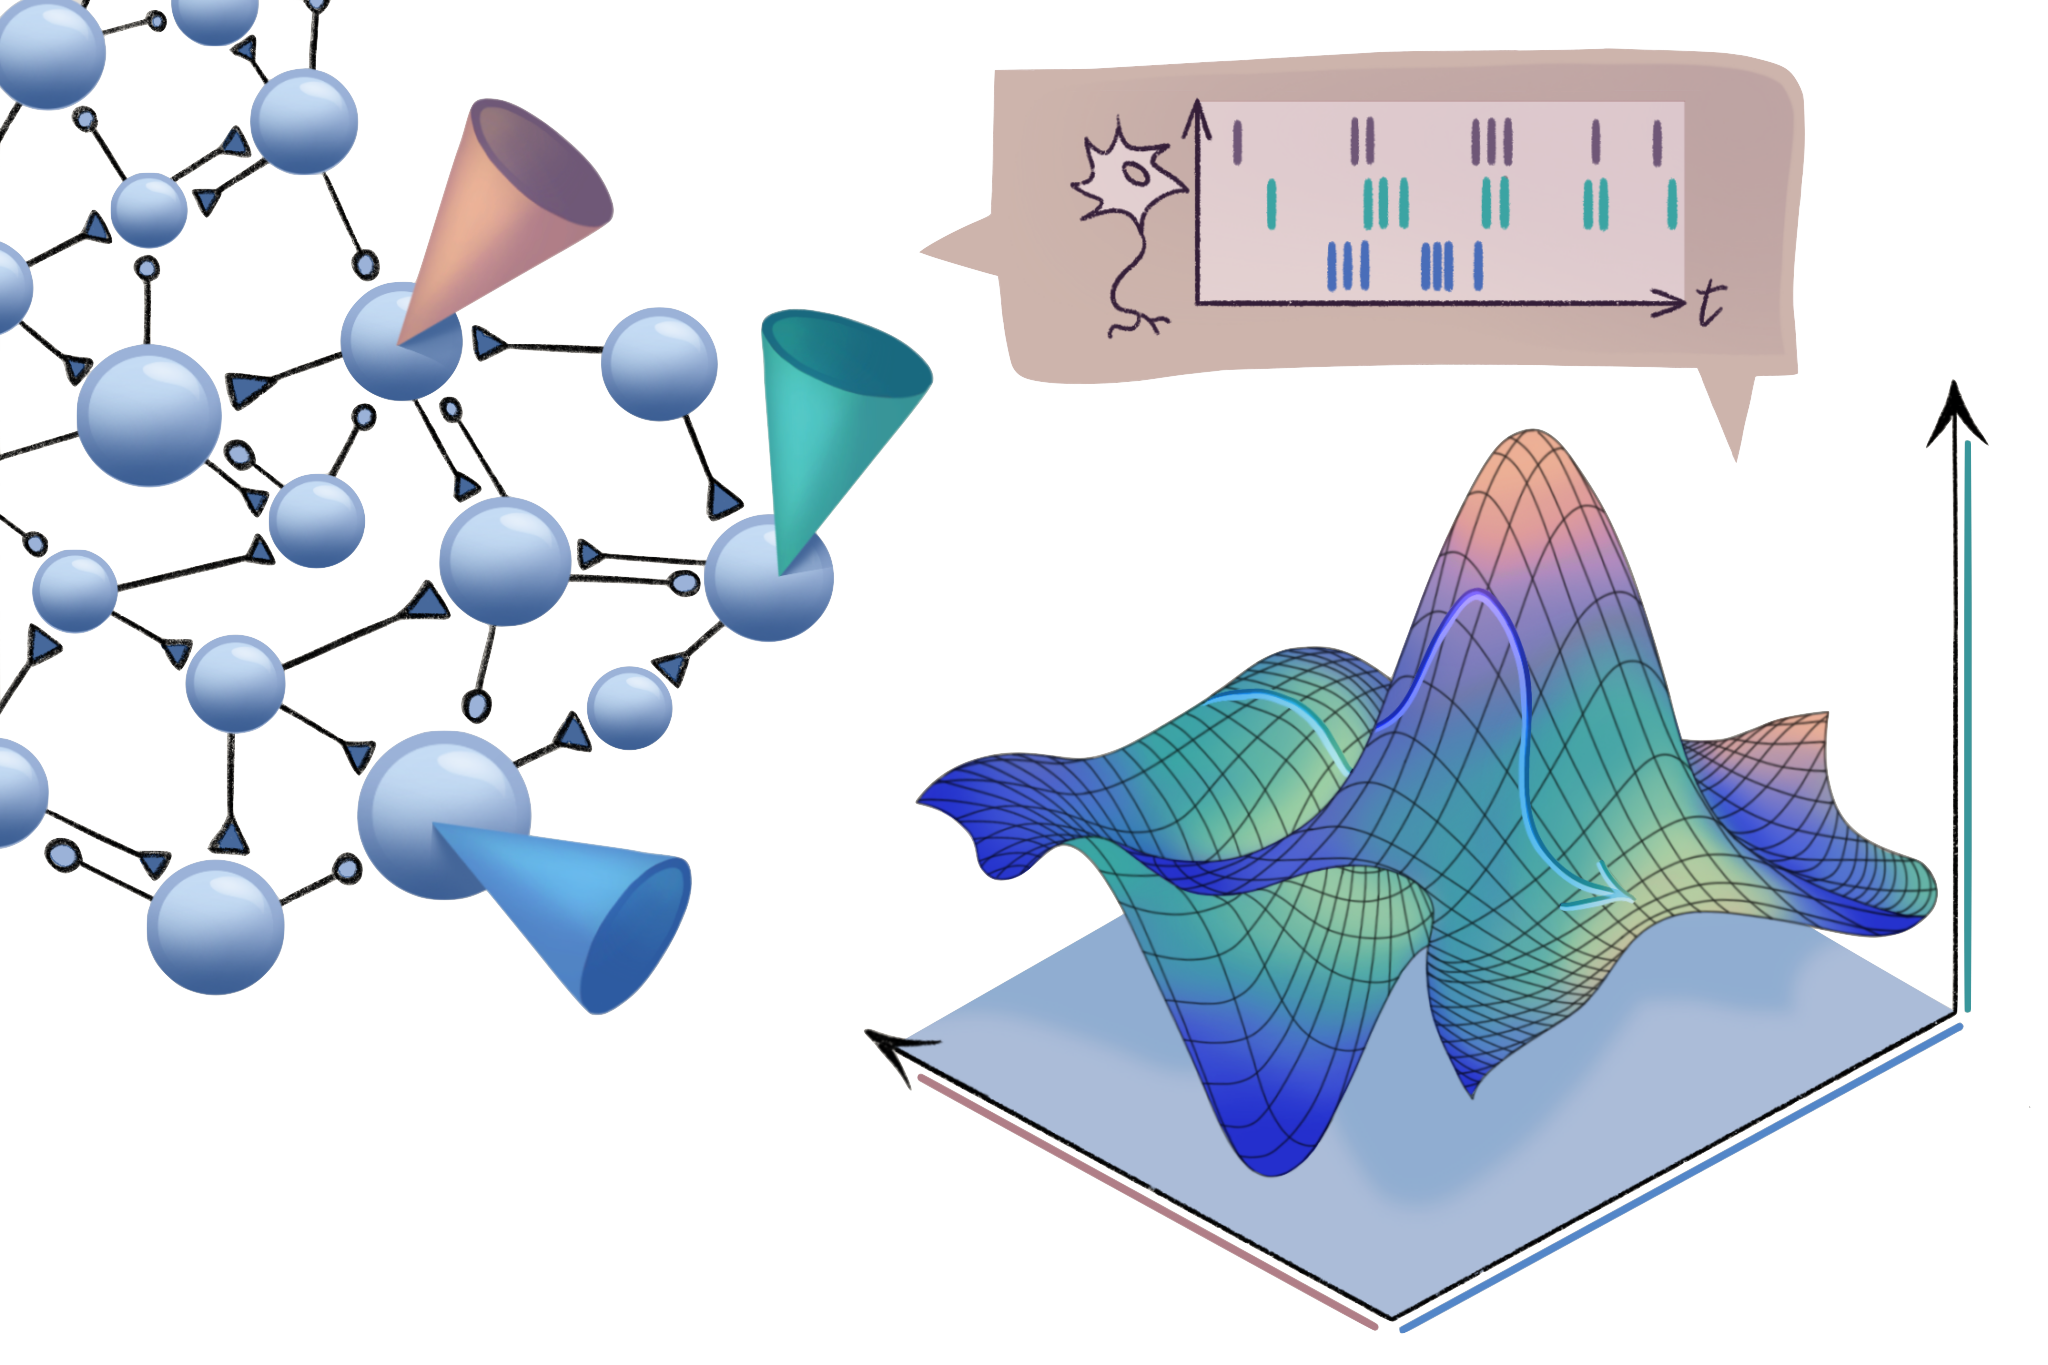
\includegraphics[width=0.75\linewidth]{manifold_schematic.png}
    \caption{A neural manifold is formed by plotting neural activity (e.g., firing rate) in state space, where each axis is a single neuron. Note that the repeated presentation of the same stimulus does not lead to the occupancy of an identical point within the state space. Rather, neuronal variability induces fluctuations in the points derived from different trials. Consequently, each stimulus is associated not with a single point but with a point cloud, the dimensions and configuration of which are contingent upon the magnitude and nature of the neuronal variability. One may be interested in the manifold that emerges in response to a particular stimulus or whether there is separability among manifolds from multiple stimuli. Figure from \cite{Perich2024}.}
    \label{fig:manifolds}
\end{figure}


\section{Neural Population Geometry}

\section{Mouse Experiment}

\section{Simulation Study}

To demonstrate the emergence of geometric structures in neural representations of ANNs, we implemented a simulation experiment investigating how ANNs encode ``circular variables''. This experiment provides an example of neural population geometry principles and illustrates how topological structures may naturally emerge in neural representations.


We trained a convolutional neural network (CNN) to predict the orientation of visual grating stimuli, a task analogous to orientation selectivity in the visual cortex. The network was presented with sinusoidal gratings at various orientations ranging from 0° to 360° and tasked with predicting the orientation angle.

\begin{figure}
    \centering
    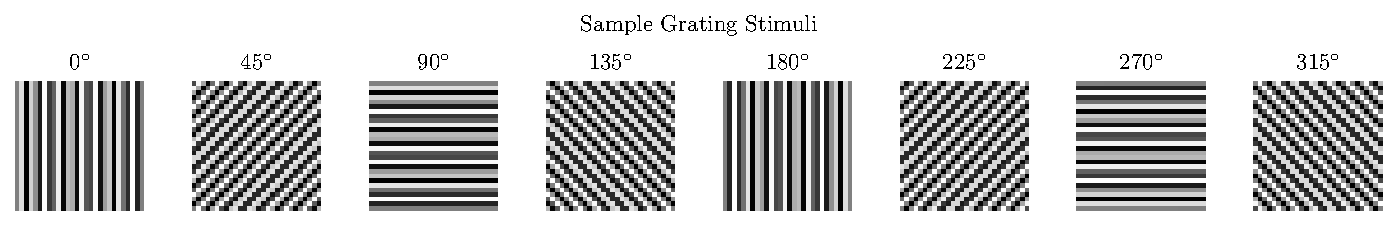
\includegraphics[width=\linewidth]{results/grating_samples.pdf}
    \caption{Sample grating stimuli at different orientations.}
    \label{fig:grating_samples}
\end{figure}

The architecture consisted of convolutional layers followed by fully connected layers, with a 32-dimensional latent space that we analyzed for geometric properties. Importantly, the network was trained to predict the sine and cosine components of the orientation angle rather than the raw angle, which naturally handles the circular topology of the orientation space (where 0° and 360° are identical).

After training, we extracted the 32-dimensional latent representations for test stimuli and applied dimensionality reduction techniques (PCA, t-SNE, and UMAP) to visualize the structure of these representations. The results revealed a striking circular manifold in the latent space, where stimuli with similar orientations were positioned close together, and the entire orientation space was represented as a continuous ring.

\begin{figure}[h]
    \centering
    \begin{subfigure}[b]{0.48\linewidth}
        \centering
        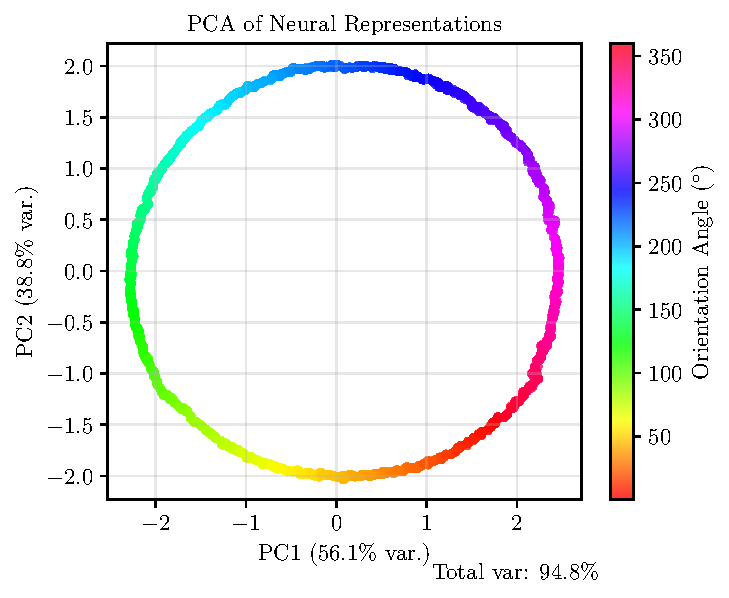
\includegraphics[width=\linewidth]{results/pca_latent_space.pdf}
        \caption{PCA of the latent space}
    \end{subfigure}
    \hfill
    \begin{subfigure}[b]{0.48\linewidth}
        \centering
        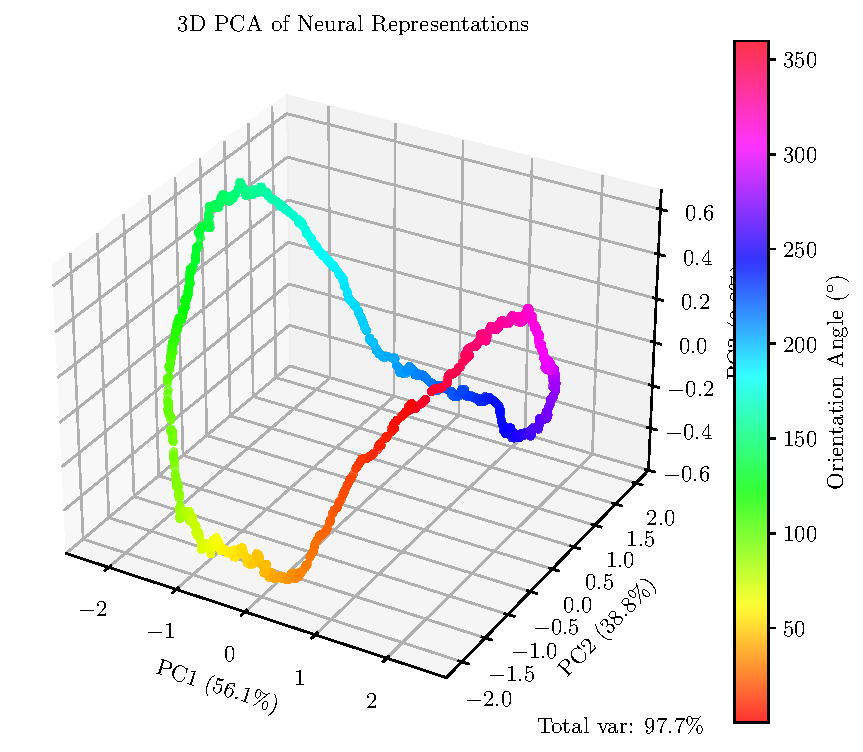
\includegraphics[width=\linewidth]{results/3d_manifold.pdf}
        \caption{3D visualization of the manifold}
    \end{subfigure}
    \caption{Visualization of the circular manifold in the neural network's latent space using different dimensionality reduction techniques.}
    \label{fig:pca_latent_space}
\end{figure}

This circular topology emerged naturally from the training process, despite no explicit topological constraints being imposed on the network. The network discovered that a circular representation is the most efficient way to encode a periodic variable, demonstrating how the geometry of the task space (in this case, the circular nature of orientation angles) becomes reflected in the geometry of the neural representations.

The experiment highlights several key principles of neural population geometry:

\begin{itemize}
    \item \textbf{Manifold structure}: The network's internal representations form a low-dimensional manifold (a circle) embedded in the high-dimensional latent space.
    \item \textbf{Topological correspondence}: The topology of the manifold (circular) matches the topology of the task space (orientation angles).
    \item \textbf{Continuous representation}: Similar stimuli are mapped to nearby points on the manifold, preserving the continuity of the input space.
    \item \textbf{Dimensionality reduction}: The network learns to compress the high-dimensional input (grating images) into a low-dimensional representation that captures the essential variable (orientation).
\end{itemize}


This simple experiment provides an intuitive foundation for understanding how more complex neural networks might represent more complicated manifolds in their latent spaces, and how the geometry of these representations relates to the computational tasks being performed.


\section{Conclusion}

\bibliographystyle{unsrt}
\bibliography{refs}

\end{document}
